%%%%%%%%%%%%%%%%%%%%%%%%%%%%%%%%%%%%%%%%%%%%%%%%%%%%%%%%%%%%%%%%%%%%%%%%%%%%%%%%%%%%%%%%%%%%%%%%%%%
% Chapter 1 -> Introduction
% Author: Eduardo G Gusmao
%%%%%%%%%%%%%%%%%%%%%%%%%%%%%%%%%%%%%%%%%%%%%%%%%%%%%%%%%%%%%%%%%%%%%%%%%%%%%%%%%%%%%%%%%%%%%%%%%%%
\chapter{Introduction}
\label{cha:introduction}

\graphicspath{{chapter1/figs/}}

%%%%%%%%%%%%%%%%%%%%%%%%%%%%%%%%%%%%%%%%%%%%%%%%%%%%%%%%%%%%%%%%%%%%%
% Section: Motivation
%%%%%%%%%%%%%%%%%%%%%%%%%%%%%%%%%%%%%%%%%%%%%%%%%%%%%%%%%%%%%%%%%%%%%
\section{Motivation}
\label{sec:problem.motivation}

\subsubsection{Gene Regulation and Transcription Factor Binding Sites}

% Genome
Every living organism is composed of multiple different cells. These cells contain genetic material encoded in the form of deoxyribonucleic acid (DNA) molecules, also known as genome. The genome can be represented as a categorical vector $\mathbf{g} = \langle g_1, \cdots, g_n \rangle$, where $g_i \in \{\text{A},\text{C},\text{G},\text{T}\}$ represents the nucleotide at genomic position $i$. Certain regions within the genome encode the so-called genes. Genes can be read by specialized proteins to produce other proteins. This protein-producing cycle is the key mechanism for maintenance of life.

% Genome is not enough
A couple of years ago, it was believed that, in possession of the complete genomic sequence $\mathbf{g}$ for a given organism, it would be possible to exactly determine its phenotype and disease susceptibility. However, after the analysis of the first genomes, it was clear that the simple determination of an organism's DNA nucleotide sequence is not enough to explain the great diversity of biological processes. Such processes are governed by a complex chain of events called ``gene regulation''. Gene regulation includes a wide range of mechanisms that happen inside a cell in which genes are turned ``on'' (i.e. they are expressed) and ``off'' (i.e. they are not expressed) dynamically. Depending on which genes are ``on'' or ``off'', the cell specializes in different functionalities~\citep{alberts2007}.

% Post-genomic era
In the so-called post-genomic era, attention is turning to the understanding of how protein-coding genes (about $25,000$ in humans) and their products are regulated~\citep{maston2006}. These regulatory mechanisms drive the correct execution of biological processes and require a set of carefully orchestrated steps that depend on the correct spatial and temporal expression of genes~\citep{maston2006}. On the other hand, the deregulation of gene expression, i.e. errors regarding the regulatory steps, is often linked to diseases~\citep{encode2012}.

% Regulatory elements
To understand the molecular mechanisms that dictate the cell's expression patterns, it is important to identify the regulatory elements involved in these activities. One of the most important regulatory players are transcription factors (TFs) -- proteins that bind on the DNA enhancing or repressing the expression of genes. These proteins bind to particular genomic regions called transcription factor binding sites (TFBSs)~\citep{maston2006}. TFBSs may be active if they are currently being bound by a TF or inactive, if they are not currently being bound by a TF.

\subsubsection{Importance of the Identification of All Active TFBSs of a Cell}

% Importance of the problem - introduction
The identification of all active TFBSs of a cell is a very important task, since they are the key players on regulatory mechanisms. By identifying active TFBSs we can develop regulatory networks, which encode the interplay between different genes to control specific cell functions. Such a task leads to the understanding of cellular mechanisms and the particular deregulatory steps which leads to disease.

% Examples
There are a great number of successful experimental studies that benefited from the proper identification of active TFBSs. For instance, studies were able to: (1) unravel cellular mechanisms~\citep{lin2015,tsankov2015}; (2) unravel disease mechanisms~\citep{schaub2012,vernot2012,charos2012}; (3) understand the function of different regions in the genome~\citep{yip2012,whitfield2012,natarajan2012} and (4) understand other cellular regulatory elements such as long noncoding ribonucleic acids (lncRNAs)~\citep{tilgner2012,banfai2012}.

% Our research goal
In summary, the identification of active transcription factor binding sites is important because of its broad impact on many other cellular processes. Given the importance of the proper identification of cell-specific active TFBSs, our research focuses on performing such a task by applying computational methods to biological experimental data.

\subsubsection{Computational Detection of Active TFBSs Must Consider the Chromatin Dynamics}

% Sequence-based methods
Historically, the first computational approach to identify TFBSs was based solely on the DNA sequence~\citep{stormo2000}. Each TF has a particular DNA sequence affinity, i.e. they tend to bind to specific DNA sequences. The computational sequence-based methods search the genome $\mathbf{g}$ for DNA substrings that correspond to the affinity sequence of target TFs. However, although computational sequence-based methods are able to detect TFBSs, they are not able to tell whether these sites are active or inactive~\citep{pique2011}. This happens because such computational approach does not consider the fact that only a few regions in the genome are accessible for TFs to bind. These regions are called ``open chromatin regions''. The number of open chromatin regions and their location vary between different cell types and ultimately dictates which genes are accessible and being expressed~\citep{encode2012}.

% NGS techniques
Recent advances in biological techniques~\citep{shendure2008} have enabled the creation of experimental methods to identify these open chromatin regions~\citep{encode2012}. We will explore two of these so-called ``open chromatin next-generation sequencing (NGS) techniques'': the chromatin immunoprecipitation followed by NGS -- termed ChIP-seq~\citep{johnson2007}; and the DNase I cleavage followed by NGS -- termed DNase-seq~\citep{crawford2004,sabo2004a}. These techniques generate time series-like signals which span the entire genome and indicate open chromatin regions. These signals can be viewed as a numeric vector $\mathbf{x} = \langle x_1, \cdots, x_n \rangle$ where high data points $x_i \in {\mathbb{N}}^{0}$ indicate open chromatin regions. Moreover, certain patterns in the signals generated by DNase-seq and ChIP-seq are indicative of active TFBSs. Therefore, we can apply computational methods to process the DNase-seq and ChIP-seq signals and to identify these patterns. By doing so, we can detect active TFBSs considering the open chromatin information.

\subsubsection{Computational Detection of Active TFBSs Using DNase-seq and ChIP-seq}

% Histone modification ChIP-seq and DNase-seq
The DNA is found wrapped in proteins called histones. There are a number of post-translational modifications on these histones which are indicative of open chromatin regions, such as the so-called H3K4me1 and H3K4me3. By performing a histone modification ChIP-seq experiment we are able to identify cell-specific open chromatin regions. Furthermore, the DNase-seq data also provides a robust map of open chromatin regions with a very high spatial resolution. By combining these two experimental data, we observe very characteristic patterns indicating the active binding of TFs in the genome (Figure~\ref{fig:gusmao_tfbs_pattern}). This pattern is commonly referred to as TF ``footprints''. A TF footprint is defined as a region likely to be represent an active TFBS~\citep{boyle2011,gusmao2012}.

% Computational footprinting methods
The experiments presented in this thesis focus on the computational treatment of DNase-seq and histone modification ChIP-seq data to perform computational predictions of active transcription binding sites. Such prediction is performed by searching the distinctive patterns, i.e. footprints, that the DNase-seq and histone modification ChIP-seq signals exhibit around active TFBSs. We use the traditional term ``computational footprinting methods'' for computational methods that searches for footprints using open chromatin data, such as DNase-seq and histone modification ChIP-seq. The computational footprinting framework presented in this thesis can be used in multiple different biological experiments to understand the regulation of genes.

% Figure - Distinctive pattern of DNase-seq and ChIP-seq on active TFBSs
\begin{figure}[h!]
\centering
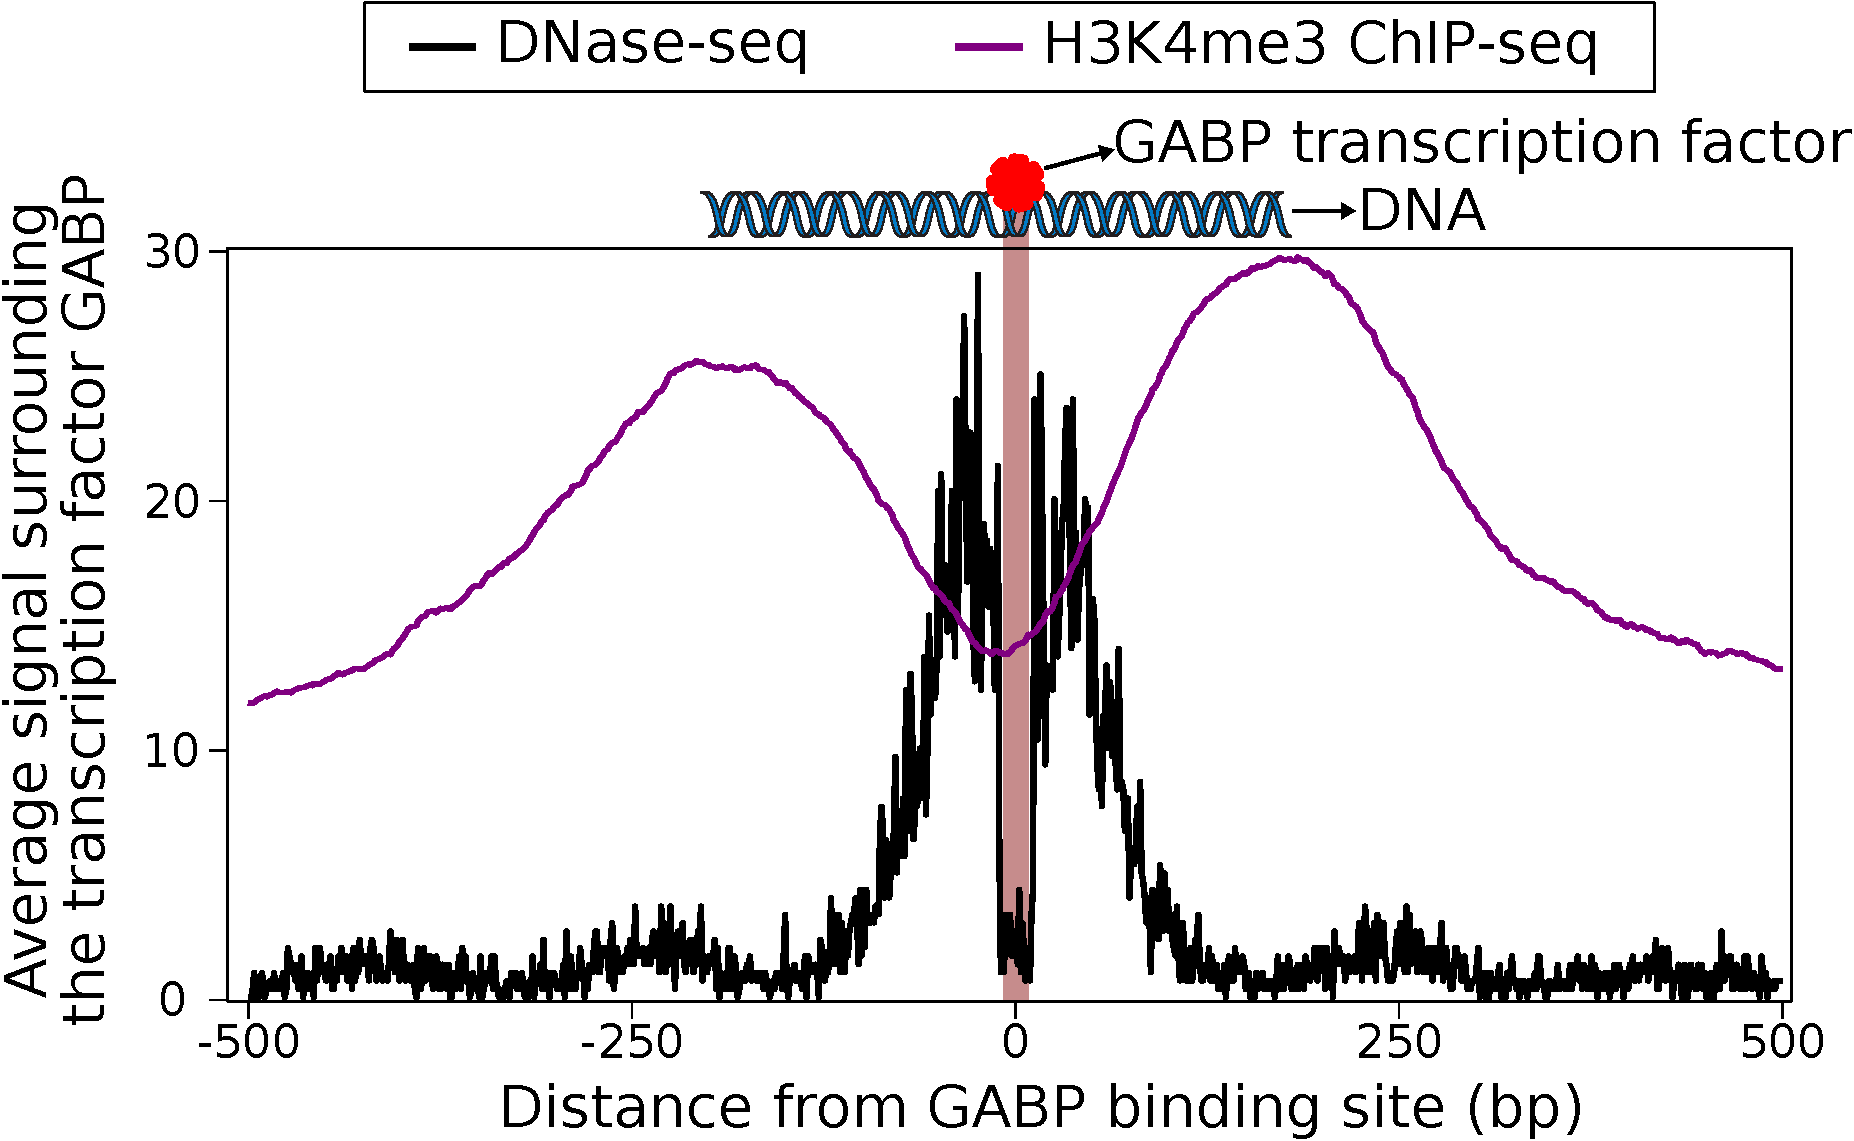
\includegraphics[width=0.8\textwidth]{gusmao_tfbs_pattern}
\caption[Distinctive pattern (footprint) of DNase-seq and ChIP-seq on active TFBSs]{\textbf{Distinctive pattern (footprint) of DNase-seq and ChIP-seq on active TFBSs.} Average DNase-seq and histone modification H3K4me3 ChIP-seq signals surrounding the known (biologically verified) TF GABP active binding sites. Active TFBSs happen at depletions between two peaks of the DNase-seq signal (marked in red). Furthermore, these DNase-seq peaks, which determines an open chromatin region, happen at the depletion between two peaks of active histone modification marks. This distinctive pattern of signal depletion between two peaks is called a TF footprint. \emph{Source:~\cite{gusmao2012}} (modified to fit thesis format and/or clarify key points).}
\label{fig:gusmao_tfbs_pattern}
\end{figure}

%%%%%%%%%%%%%%%%%%%%%%%%%%%%%%%%%%%%%%%%%%%%%%%%%%%%%%%%%%%%%%%%%%%%%
% Section: Thesis Overview
%%%%%%%%%%%%%%%%%%%%%%%%%%%%%%%%%%%%%%%%%%%%%%%%%%%%%%%%%%%%%%%%%%%%%
\section{Thesis Overview}
\label{sec:thesis.overview}

% Nutshell
In this thesis, we: (1) present a novel computational framework that uses DNase-seq and histone modification ChIP-seq data to detect active TFBSs, (2) evaluate the predictions made by our method using experimentally verified active TFBSs and (3) use our predictions in real biological scenarios to make inferences about the regulatory circuitry of particular cells. Figure~\ref{fig:gusmao_thesis_overview} presents an overview of this thesis. In the following paragraphs we describe the Figure~\ref{fig:gusmao_thesis_overview} in more detail.

\subsubsection{Computational Footprinting Framework}

% Our approach 1
For a particular cell type $A$ we obtain DNase-seq and histone modification ChIP-seq data available in repositories such as the~\cite{encode2012} (Figure~\ref{fig:gusmao_thesis_overview}a). We process these data using computational methods (Figure~\ref{fig:gusmao_thesis_overview}b) to generate a normalized DNase-seq signal $\mathbf{x}_A$ and normalized histone modification ChIP-seq signal $\mathbf{y}_A$ (Figure~\ref{fig:gusmao_thesis_overview}c). Then, we apply a computational footprinting method $\Theta$ on $\mathbf{x}_A$ and $\mathbf{y}_A$ (Figure~\ref{fig:gusmao_thesis_overview}d) generating a set of genomic regions (intervals) $S_A = \{s_{A1}, \cdots, s_{Am}\}$, where each genomic interval $s_{Ai} = [u,v]$ represent a predicted footprint, which is likely to be associated to an active TFBS (Figure~\ref{fig:gusmao_thesis_overview}e).

\subsubsection{Evaluation of Predicted Footprints}

% Our approach 2
The predicted footprints $S_A$ are compared to experimentally verified active TFBSs (Figure~\ref{fig:gusmao_thesis_overview}e) to create statistics which evaluate how close our predictions are to the true active TFBSs (Figure~\ref{fig:gusmao_thesis_overview}f-g). These evaluation statistics (Figure~\ref{fig:gusmao_thesis_overview}g) are also used to compare our computational footprinting framework to competing methodologies. 

\subsubsection{Application to Real Biological Scenarios}

% Our approach 3
Furthermore, the predicted footprints $S_A$ are used in combination with downstream computational methods (Figure~\ref{fig:gusmao_thesis_overview}i) to generate real-scenario biological knowledge about the regulatory circuitry of the cell type $A$ (Figure~\ref{fig:gusmao_thesis_overview}j).

% Figure - Thesis overview
\begin{figure}[h!]
\centering
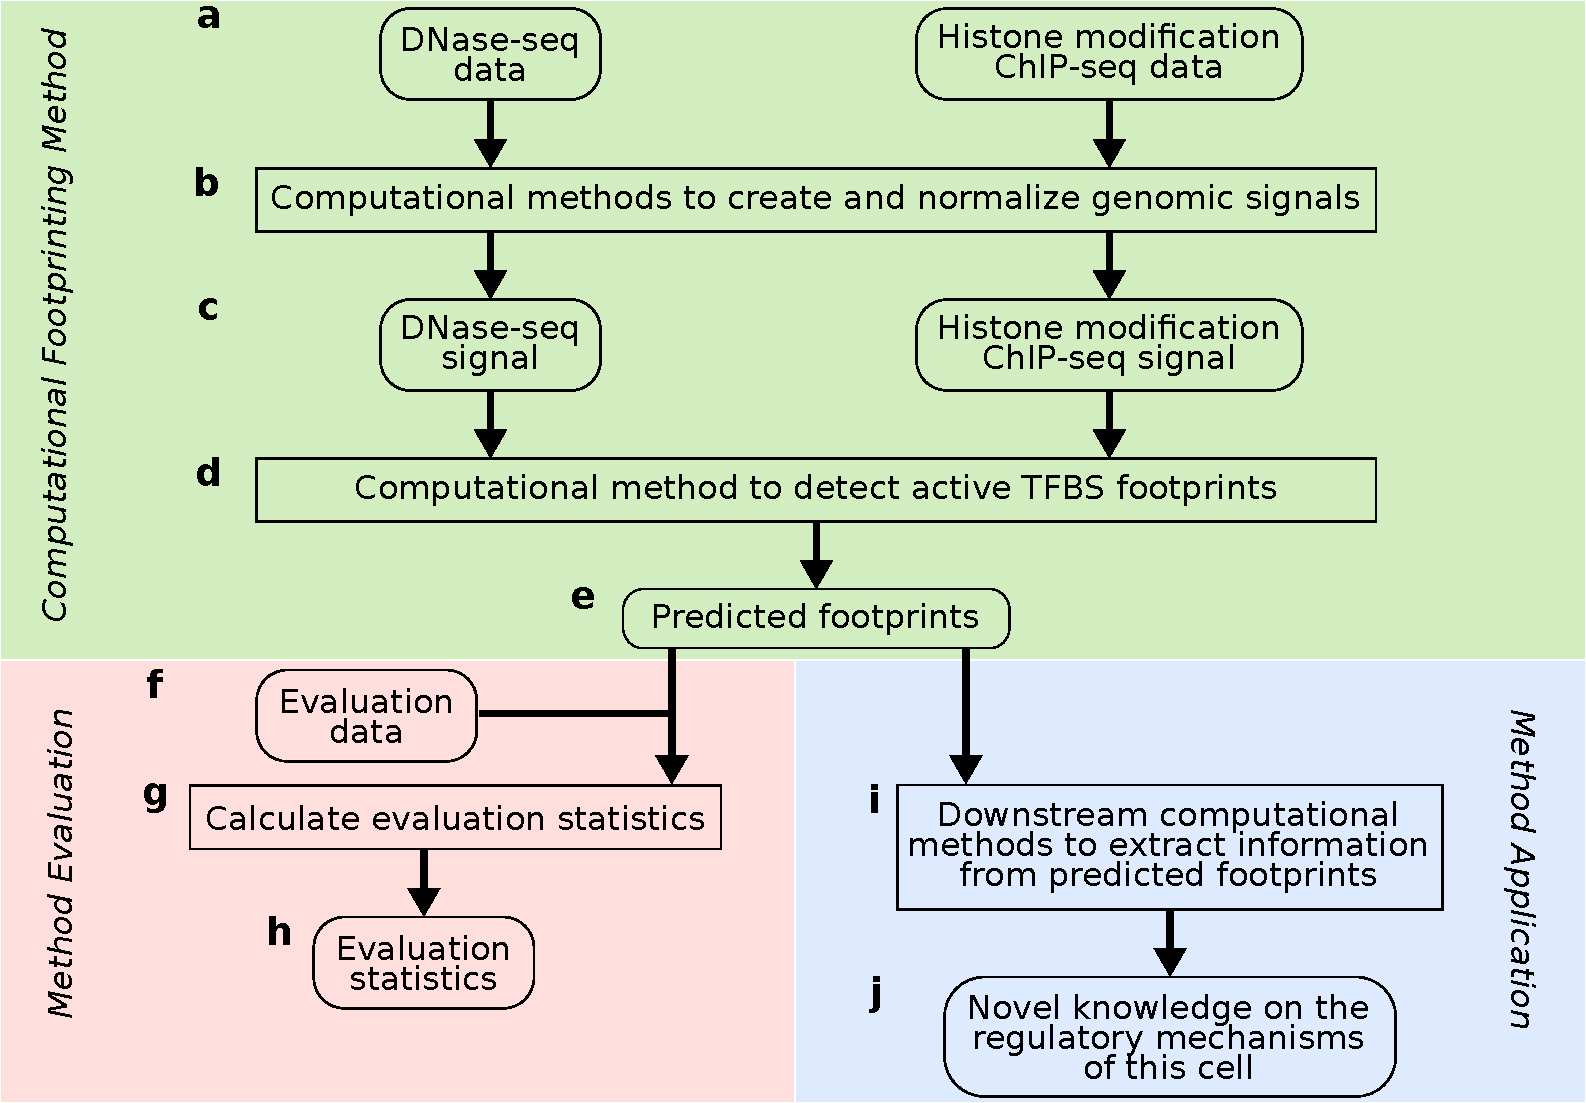
\includegraphics[width=0.95\textwidth]{gusmao_thesis_overview}
\caption[Thesis overview]{\textbf{Thesis overview.} This figure depicts the proposed thesis' workflow. Boxes with round-shaped edges represent data and square-shaped edges represent computational methods.}
\label{fig:gusmao_thesis_overview}
\end{figure}


%%%%%%%%%%%%%%%%%%%%%%%%%%%%%%%%%%%%%%%%%%%%%%%%%%%%%%%%%%%%%%%%%%%%%
% Section: Contributions
%%%%%%%%%%%%%%%%%%%%%%%%%%%%%%%%%%%%%%%%%%%%%%%%%%%%%%%%%%%%%%%%%%%%%
\section{Contributions}
\label{sec:contributions}

% Framework to analyze active TFBSs
The main contribution of this work is the development of a novel computational framework to treat data generated with the DNase-seq and ChIP-seq technologies and detect footprints (i.e. putative active TFBSs) based on these data. Our contributions are summarized as follows.

% Contributions
\begin{itemize}
  \item \textbf{Novel computational footprinting method:} We devised a novel computational footprinting method based on hidden Markov models (HMMs). Our novel methodology is the first to successfully combine DNase-seq and histone modification ChIP-seq to predict footprints, i.e. putative active TFBSs. Such method was shown to provide robust active TFBS predictions on the basis of an extensive evaluation process.
  \item \textbf{Novel signal treatment strategy:} Novel DNase-seq and histone modification ChIP-seq signal treatment approaches were developed and formalized. Such treatment framework has shown to be robust and applicable to a wide range of different datasets.
  \item \textbf{DNase-seq experimental bias correction:} We created an approach to correct for known artifacts on DNase-seq data. Our experiments have shown the efficiency of such correction on bias mitigation.
  \item \textbf{Novel evaluation approach of computational footprinting methods:} Until now, computational footprinting methods have been evaluated using the ``TF ChIP-seq approach''. However, biases were pointed in such evaluation scheme~\citep{yardimci2014}. Therefore, we develop a novel computational footprinting method evaluation approach based on gene expression.
  \item \textbf{Comprehensive computational footprinting method comparison:} We performed a comprehensive comparison including: (1) our novel HMM-based approach; (2) nine state-of-the-art computational footprinting methods and (3) four baseline approaches. Our comparative experiment is the most complete so far, with a total of $14$ computational footprinting methods and $233$ TFs evaluated.
  \item \textbf{Analysis of relevant features on computational footprinting:} A number of empirical analyses were performed. These analyses evaluated relevant features for the computational prediction of active TFBSs such as: method's parameter selection, experimental bias correction, optimal footprint scoring strategy and TF binding residence time.
  \item \textbf{Case studies:} We successfully applied our computational footprinting method in two different studies to identify regulatory elements involved in specific biological conditions.
\end{itemize}

%%%%%%%%%%%%%%%%%%%%%%%%%%%%%%%%%%%%%%%%%%%%%%%%%%%%%%%%%%%%%%%%%%%%%
% Section: Document Structure
%%%%%%%%%%%%%%%%%%%%%%%%%%%%%%%%%%%%%%%%%%%%%%%%%%%%%%%%%%%%%%%%%%%%%
\section{Document Structure}
\label{sec:document.structure}

% Chapter 2
In Chapter~\ref{cha:background} we introduce all the concepts needed for the understanding of our work. We define the current challenges on computational identification of active TFBSs and provide a comprehensive literature review on computational footprinting methods.

% Chapter 3 / 4
In Chapter~\ref{cha:methods} we formalize our approach to address the detection of active TFBSs. We describe the treatment of the input DNase-seq and ChIP-seq data and the novel approach to detect active TFBSs based on HMMs. Furthermore, in Chapter~\ref{cha:experiments} we describe the full experiment design of this project. We present the data used in our work, the execution of our computational footprinting approach and method evaluation strategies.

% Chapter 5 / 6
In Chapter~\ref{cha:results} we present the results of our experiments, which encompasses: the analyses on relevant computational footprinting features, a comprehensive comparison of computational footprinting methods and case studies in which our methodology was successfully applied to real biological scenarios. In Chapter~\ref{cha:conclusion} we discuss all results presented in this thesis, highlighting all the key findings. Furthermore, we discuss future research opportunities. Further supplementary information and results can be found in the Appendix~\ref{cha:appendix}.


